\chapter{Thermal noise and nucleation}
\label{ch:p8}

\begin{keybox}
\textbf{Key idea.} Where do the crystal seeds of Chapter~\ref{ch:p6} come
from? From thermal \emph{fluctuations}. An undercooled melt is
\emph{metastable}: $\psi=0$ sits behind a free-energy barrier, and the
crystal cannot form until a fluctuation pushes a small region over that
barrier --- classical nucleation. Here the noise is \emph{physics}, and
its amplitude ($k_BT$) sets the nucleation rate. Getting the DISCRETE
fluctuation--dissipation normalization right --- and \emph{verifying} it
numerically --- is the heart of this chapter.
\end{keybox}

\section{The model and the discrete FDT normalization}

We add the physical (fluctuation--dissipation) noise to the Allen--Cahn
crystallinity equation:
%
\begin{equation}
  \dd{\psi}{t} = -L_\psi\Big[\dd{f}{\psi}-\varepsilon^2\grad^2\psi\Big]
   + \xi,\qquad
  \langle\xi(\mathbf{x},t)\,\xi(\mathbf{x}',t')\rangle
   = 2L_\psi\,k_BT\,\delta(\mathbf{x}-\mathbf{x}')\delta(t-t').
\end{equation}
%
On the finite-element mesh the load-only forcing is drawn per Gauss point
with standard deviation
%
\begin{equation}
  \mathrm{std}(\xi_{gp}) = \texttt{noise\_psi}\,
     \sqrt{\tfrac{2 L_\psi}{\Delta t\,w^J_{gp}}},
     \qquad \texttt{noise\_psi}^2 = k_BT,
  \label{eq:p8fdt}
\end{equation}
%
where $w^J_{gp}$ is the Gauss-point quadrature weight. The two factors are
not cosmetic: the $1/\Delta t$ makes the white-noise time increment
consistent, and the $1/w^J_{gp}$ is the \emph{spatial} white-noise
quadrature normalization, so the assembled nodal force
$b_a=\int N_a\,\xi\,\dV$ has variance
%
\begin{equation}
  \mathrm{Var}(b_a) = 2\,\texttt{noise\_psi}^2\,L_\psi
     \int N_a^2\,\dV \;/\;\Delta t
\end{equation}
%
\emph{exactly} --- independent of how finely the mesh samples space. A
mesh-blind noise would make this scale with the element size and the
equilibrium fluctuations would \emph{not} converge under refinement.

\begin{keybox}
\textbf{Central verification (not a footnote).} Fix the physical noise
$k_BT$, put $\psi$ in a STABLE quadratic well (a superheated, clip-free
$r14$ well so fluctuations are two-sided and un-rectified), and measure
the equilibrium spatial variance $\langle\mathrm{Var}\,\psi\rangle$.
Equipartition predicts a value set by $k_BT$ and the well/mesh,
\emph{independent} of $\Delta t$. Refining $\Delta t$ the measured variance
converges to a $\Delta t$-independent plateau (measured coefficient of
variation across $\Delta t$: $\ensuremath{\PeightDtCov}$); refining the
mesh, $\mathrm{Var}\,\psi\cdot V_{\rm cell}$ stays constant (CoV
$\ensuremath{\PeightMeshCov}$, i.e. $\mathrm{Var}\,\psi\propto1/V_{\rm cell}$
as equipartition demands). The physical statistic converges --- the
Eq.~\eqref{eq:p8fdt} normalization is correct.
\end{keybox}

\section{Nucleation as an ensemble}

Nucleation is a random, rare-event, barrier-crossing process (rate
$\sim\exp(-\Delta F^\star/k_BT)$), so a single seed is one \emph{sample},
not a result. We run several noise realizations per amplitude and report,
via \code{diffsim.diagnostics.stochastic}, the nucleation
\emph{probability}, the crystalline-fraction distribution, the nuclei
\emph{density}, and the induction time (a first-passage crossing of
$X=0.02$), each as a mean with a $95\%$ interval.

\begin{keybox}
\textbf{Noise-amplitude sweep, NOT a temperature sweep.} We vary
\emph{only} \code{noise\_psi} ($=\sqrt{k_BT}$ in the forcing) at
\emph{fixed} undercooling $T/T_m$. A genuine temperature change would also
move the driving force and the barrier ($\text{drive}=\Delta h(1-T/T_m)$,
the entropy, the mobility); read this as a noise-amplitude / FDT-calibration
sensitivity. \textbf{Clipping is quantified}: the undercooled runs clip
$\psi\in[0,1]$, and we report the saturated ($\psi>0.99$) fraction; the
$\psi=0$ floor rectifies sub-barrier fluctuations --- exactly why the
quantitative FDT test above uses the clip-free well. (BDF1 only: the brick
asserts noise off under BDF2.)
\end{keybox}

\section{Run it}

\begin{runbox}
\textbf{Run it.}
\begin{lstlisting}
cd physics/08_noise_nucleation
python run.py            # FDT verification + nucleation ensemble + checks
\end{lstlisting}
It runs the central FDT verification and the noise-amplitude ensemble
sweep, writes \file{outputs/results.json}, and checks it against
\file{baseline.yaml}. Compare with \file{EXPECTED.md} and the figures.
\end{runbox}

\paragraph{What you should see.} The equilibrium variance is
$\Delta t$-independent (CoV $\ensuremath{\PeightDtCov}$) and scales as
$1/V_{\rm cell}$ (CoV $\ensuremath{\PeightMeshCov}$) --- the FDT
normalization checks out. With zero noise the melt stays amorphous
($X=\ensuremath{\PeightXzero}$: no nucleation). At the largest amplitude
($\texttt{noise\_psi}=\ensuremath{\PeightNoiseHi}$) the ensemble
($\ensuremath{\PeightSeeds}$ seeds) nucleates with probability
$\ensuremath{\PeightProbHi}$, reaching $X=\ensuremath{\PeightXhi}\pm
\ensuremath{\PeightXhiSd}$ in $\ensuremath{\PeightDensHi}$ nuclei (a
saturated fraction $\ensuremath{\PeightClipHi}$). More noise nucleates more
grains.

% --- generated by gen_figures.py ---
\begin{figure}[h]\centering
  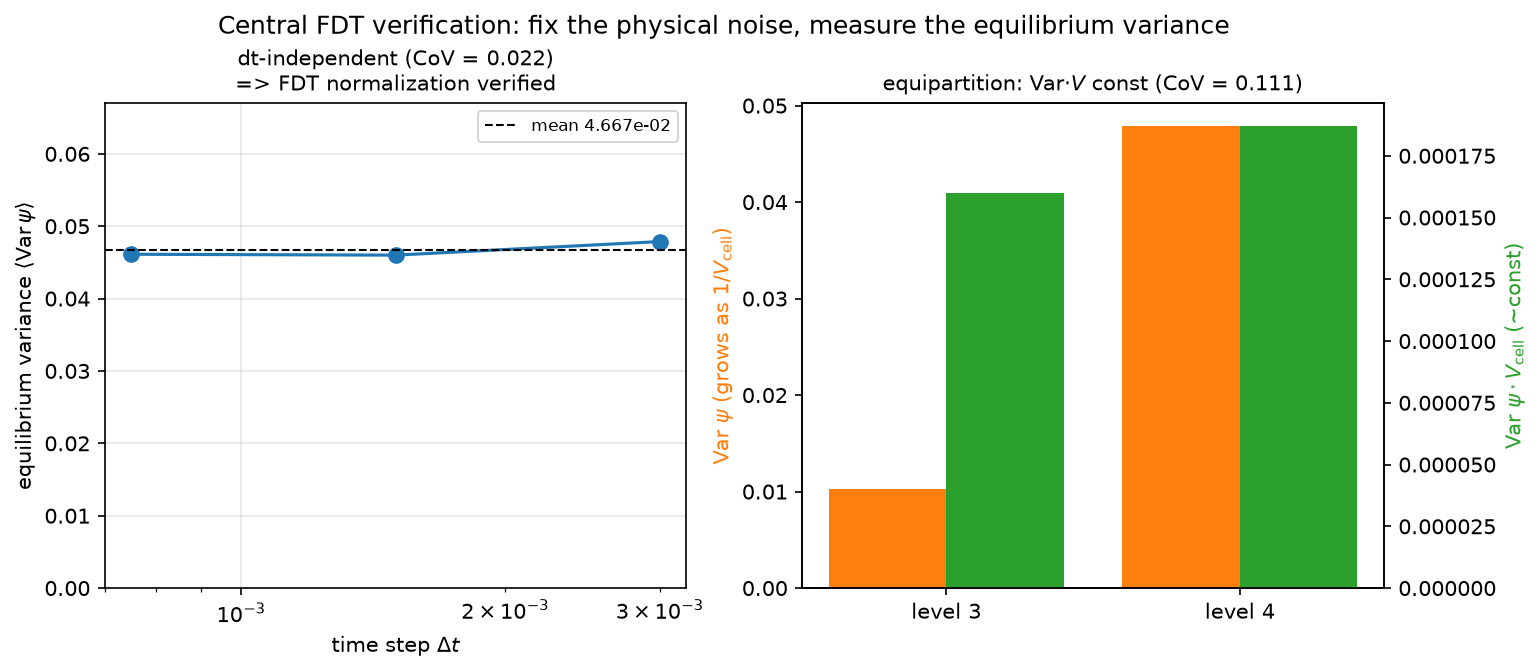
\includegraphics[width=\linewidth]{figures/p8_fdt.png}
  \caption{The central FDT verification. Left: the equilibrium variance is
    $\Delta t$-independent (a wrong $1/\Delta t$ normalization would tilt
    the line). Right: across meshes $\mathrm{Var}\,\psi$ grows as
    $1/V_{\rm cell}$ while $\mathrm{Var}\,\psi\cdot V_{\rm cell}$ stays
    constant --- equipartition.}
  \label{fig:p8fdt}
\end{figure}

\begin{figure}[h]\centering
  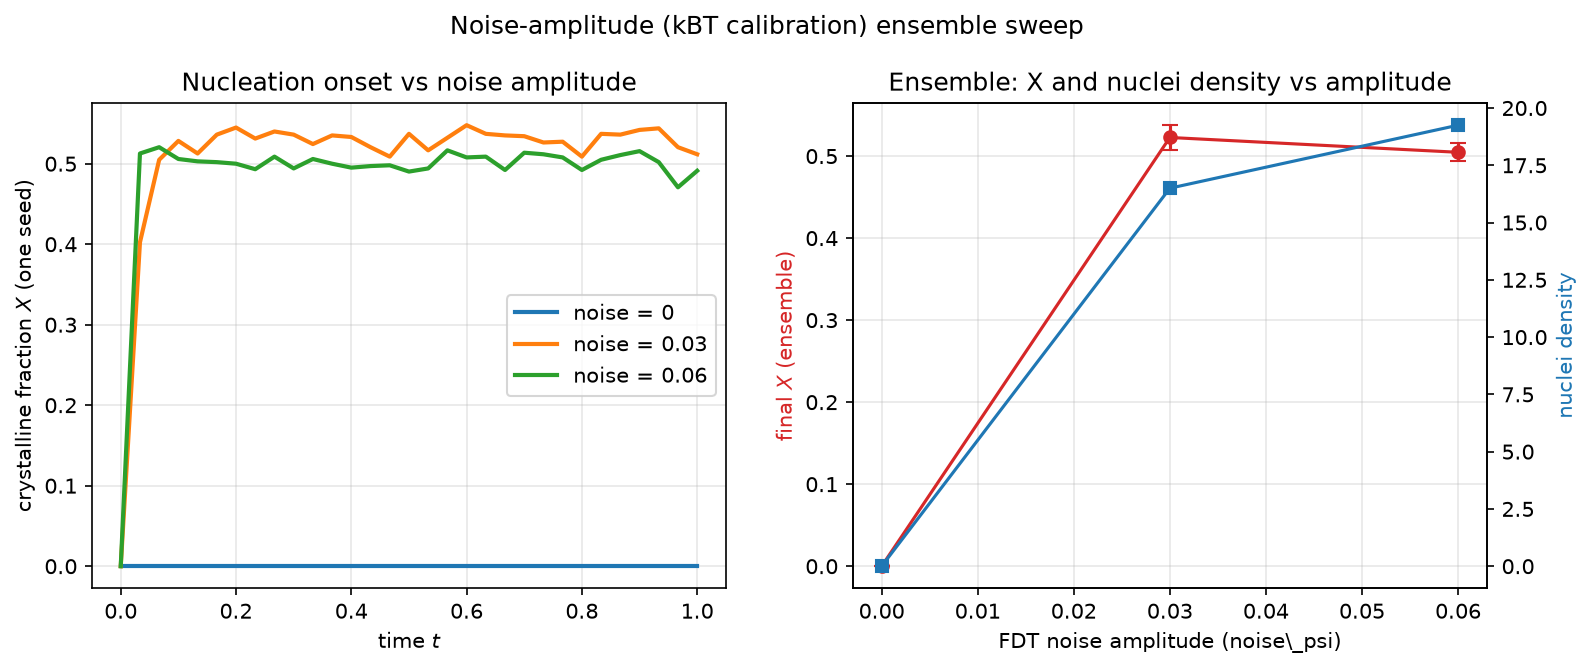
\includegraphics[width=\linewidth]{figures/p8_sweep.png}
  \caption{The noise-amplitude ensemble sweep. Left: $X(t)$ for a
    representative seed at each amplitude (zero noise never nucleates).
    Right: the ensemble final $X$ (mean $\pm$ sd) and the nuclei density
    vs amplitude.}
  \label{fig:p8sweep}
\end{figure}

\begin{figure}[h]\centering
  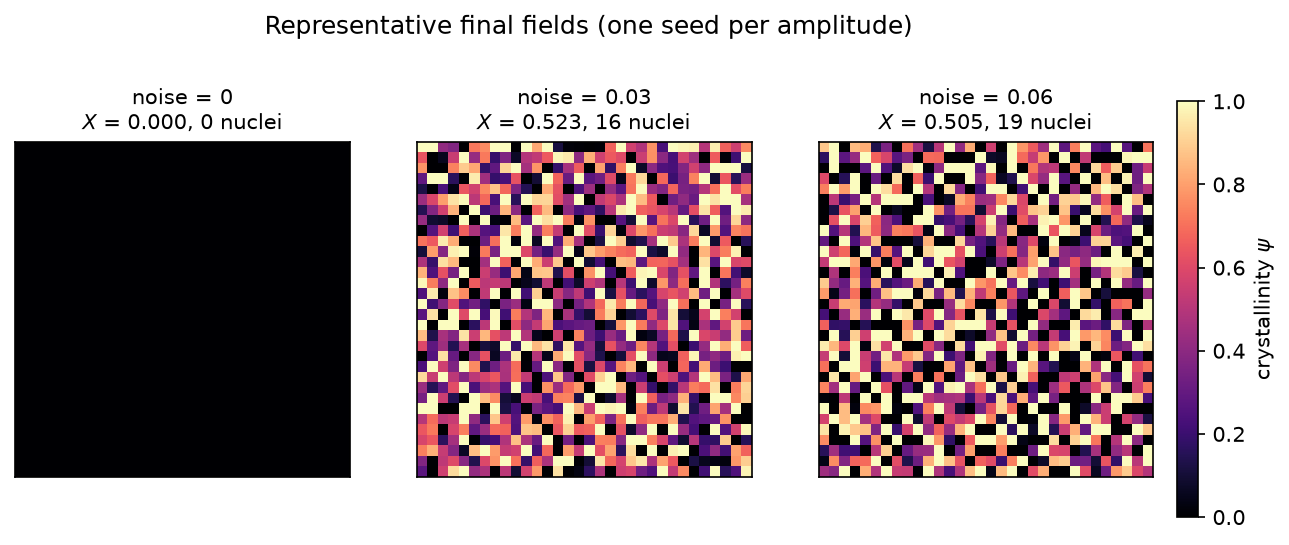
\includegraphics[width=\linewidth]{figures/p8_fields.png}
  \caption{Representative final crystallinity fields (one seed per
    amplitude): more noise nucleates more grains at fixed undercooling.}
  \label{fig:p8fields}
\end{figure}

\begin{keybox}
\textbf{Measured self-check} (tolerance-checked in \file{baseline.yaml}).
\begin{center}\small
\begin{tabular}{lc}
\toprule
FDT variance $\Delta t$-CoV / mesh-CoV & $\ensuremath{\PeightDtCov}$ / $\ensuremath{\PeightMeshCov}$ \\
zero-noise $X$ & $\ensuremath{\PeightXzero}$ \\
$X$ at $\texttt{noise\_psi}=\ensuremath{\PeightNoiseHi}$ ($\ensuremath{\PeightSeeds}$ seeds) & $\ensuremath{\PeightXhi}\pm\ensuremath{\PeightXhiSd}$ \\
nuclei density / nucleation prob. & $\ensuremath{\PeightDensHi}$ / $\ensuremath{\PeightProbHi}$ \\
\bottomrule
\end{tabular}
\end{center}
\end{keybox}

\section{Code walk-through}

\paragraph{1. The FDT verification.} \code{verify\_fdt} builds a stable
clip-free $r14$ well on a coarse CPU/splu mesh, sweeps $\Delta t$ (and the
mesh), and returns the variance CoVs --- the Eq.~\eqref{eq:p8fdt} check.

\paragraph{2. Turn on the FDT noise.} \code{MultiPhaseStepper(..., }
\code{tstep="bdf1", noise\_psi=..., noise\_seed=...)}; \code{noise\_psi} is
$\sqrt{k_BT}$, \code{noise\_seed} fixes the realization.

\paragraph{3. The ensemble sweep.} \code{run\_ensemble} runs many seeds per
amplitude and aggregates (probability, $X$, nuclei density, first-passage
induction) with CIs via \code{diffsim.diagnostics.stochastic}; the
saturated-$\psi$ fraction quantifies the clipping.

\section{Explore on your own}

\question{The nucleation rate should scale like $\exp(-\Delta
F^\star/k_BT)$. Lower the amplitudes toward the onset where the nucleation
\emph{probability} drops below one; plot $\ln(\text{nuclei density})$
against $1/\texttt{noise\_psi}^2$ and estimate the barrier from the slope.}

\question{Re-run \code{verify\_fdt} with the $1/w^J$ factor removed from
Eq.~\eqref{eq:p8fdt} (a mesh-blind noise). Does the equilibrium variance
now DEPEND on the mesh (fail the equipartition check)? This is the point of
the normalization.}

\question{Deepen the undercooling (lower $T$) at fixed noise. Does the
induction-time distribution shift earlier? Relate to how $\Delta F^\star$
depends on the driving force. (Remember: that IS a temperature change ---
it moves the barrier, unlike the noise-amplitude sweep.)}

\question{Change only the \code{noise\_seed}. Which is reproducible --- the
grain \emph{positions}, or the ensemble statistics? Connect to the seed
discussion of Chapter~\ref{ch:p1}: here the seed is physical, so a
different seed is a different valid sample.}

\question{Quantify the clipping vs amplitude. At what noise level does the
$\psi=0$ floor start to bias the pre-nucleation statistics, and how would
you correct for it (hint: the clip-free well)?}

% ====================================================================
